\documentclass[ngerman,hyperref={pdfpagelabels=false}]{beamer}

% -----------------------------------------------------------------------------

\graphicspath{{images/}}

% -----------------------------------------------------------------------------

\usetheme{KIT}

\setbeamercovered{transparent}
%\setbeamertemplate{enumerate items}[ball]

\newenvironment<>{KITtestblock}[2][]
{\begin{KITcolblock}<#1>{#2}{KITblack15}{KITblack50}}
{\end{KITcolblock}}

\usepackage[ngerman,english]{babel}
\usepackage[utf8]{inputenc}
\usepackage[TS1,T1]{fontenc}
\usepackage{array}
\usepackage{multicol}
\usepackage[absolute,overlay]{textpos}
\usepackage{beamerKITdefs}

\pdfpageattr {/Group << /S /Transparency /I true /CS /DeviceRGB>>}	%required to prevent color shifting withd transparent images


\title{Kolloquium Entwurfsphase RetroMachines}
\subtitle{Team B (RetroFactory)}

\author[Team B (RetroFactory)]{Team B (RetroFactory)}
\institute{Institut für Programmierparadigmen}

\TitleImage[width=\titleimagewd,height=\titleimageht]{titel}

\KITinstitute{Institut f\"ur Programmierparadigmen}
\KITfaculty{Fakult\"at f\"ur Informatik}

% -----------------------------------------------------------------------------

\begin{document}
\setlength\textheight{7cm} %required for correct vertical alignment, if [t] is not used as documentclass parameter


% title frame
\begin{frame}
  \maketitle
\end{frame}

\section{Grobaufbau App}
\begin{frame}
	\frametitle{Grobaufbau der App}
	{\center
		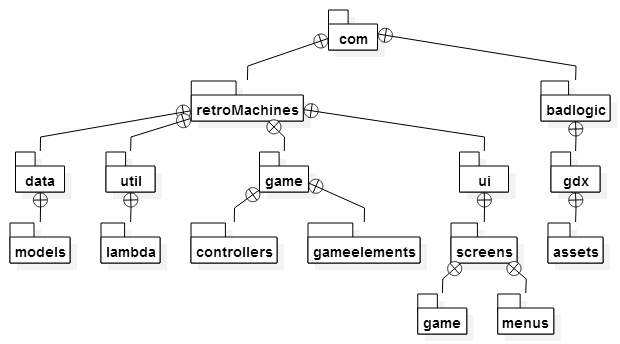
\includegraphics[scale= 0.49]{images/PackageStructure}	
		\par
	}
	\begin{itemize}
		\item Unterteilung der App in Menüs und Game
	\end{itemize}
	\bigskip
\end{frame}

\section{Aufbau Menü}
\begin{frame}
	\frametitle{Aufbau Menü}
	\begin{itemize}
		\item Screens erben von einer Klasse
		\item Design ist modular unterteilt
			\begin{itemize}
				\item Skin
				\item Font
			\end{itemize}
		\item Appstart führt ins Hauptmenü
	\end{itemize}
	\bigskip
\end{frame}

\section{Aufbau Game}
\begin{frame}
	\frametitle{Aufbau Game}
	\begin{itemize}
		\item Screens erben von einer Klasse
		\item Level bestehen aus:
		\begin{itemize}
			\item Tiled-Map
			\item JSON-File
		\end{itemize}
	\end{itemize}
	\bigskip
\end{frame}

\section{Aufbau Level}
\begin{frame}
	\frametitle{Aufbau Tiled-Map}
	{\center
		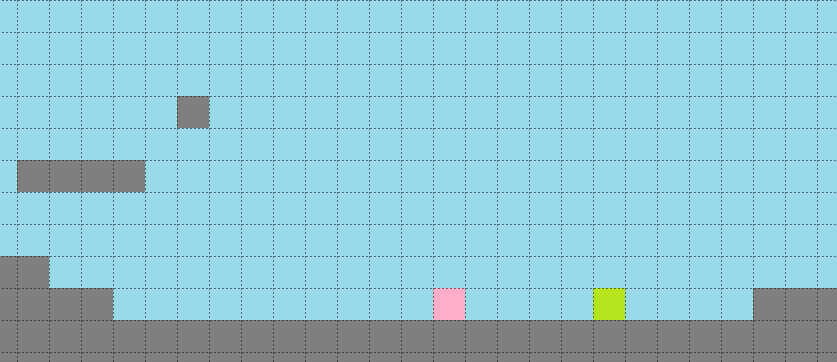
\includegraphics[scale= 0.515]{images/TiledMapBsp}
		\par
	}

	\bigskip
\end{frame}

\begin{frame}
	\frametitle{Aufbau der Tiled-Map}
	\begin{columns}[T]
		\begin{column}{4.1 cm}
			\begin{itemize}
				\item Gerastert
				\item verschiedene Ebenen
					\begin{itemize}
						\item Hintergrund
						\item Lauf-Ebene
						\item Ablagen
						\item Spielelemente
					\end{itemize}	
				\item Charakter bewegt sich vor den Ebenen
			\end{itemize}
		\end{column}
		\hfill
		\begin{column}{7 cm}
			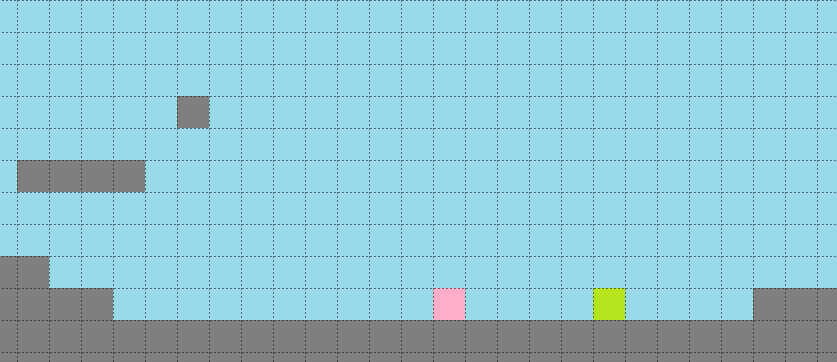
\includegraphics[scale= 0.31]{images/TiledMapBsp}
		\end{column}
	\end{columns}
	\bigskip
\end{frame}

\begin{frame}
	\frametitle{Aufbau JSON}
	{\center
		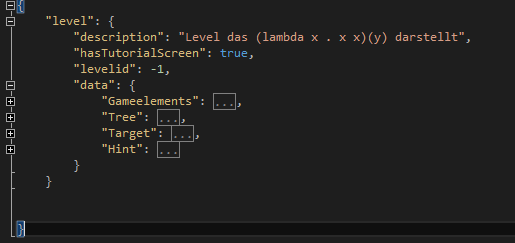
\includegraphics[scale= 0.84]{images/JsonGrob}
		\par
	}
	\bigskip
\end{frame}

\begin{frame}
	\frametitle{Aufbau JSON}
	\begin{columns}[T]
		\begin{column}{4 cm}
			\begin{itemize}
				\item Allgemeine Infos
				\item Daten
				\begin{itemize}
					\item Spielelemente
					\item Auswertungsstruktur
					\item Zielkonstellation
					\item Hinweiskonstellation
				\end{itemize}
			\end{itemize}
		\end{column}
		\hfill
		\begin{column}{7 cm}
			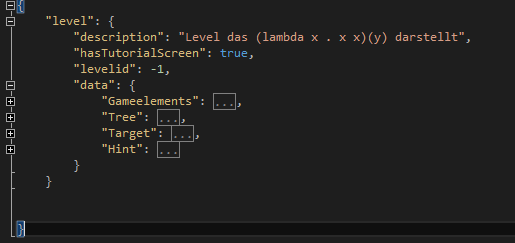
\includegraphics[scale= 0.5]{images/JsonGrob}
		\end{column}
	\end{columns}
	\bigskip
\end{frame}

\begin{frame}
	\frametitle{Aufbau JSON}
	{\center
		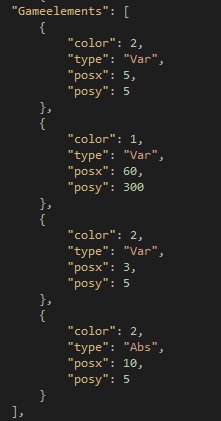
\includegraphics[scale= 0.6]{images/GameelementJson}	
		\par
	}
	\bigskip
\end{frame}

\begin{frame}
	\frametitle{Aufbau JSON}
	\begin{columns}[T]
		\begin{column}{5 cm}
			\begin{itemize}
				\item Liste aller Spielelemente
				\item Attribute
				\begin{itemize}
					\item color: Elementgruppe
					\item type: Element Typ
					\item posx: Position X-Achse
					\item posy: Position Y-Achse
				\end{itemize}
			\end{itemize}
		\end{column}
		\hfill
		\begin{column}{5 cm}
			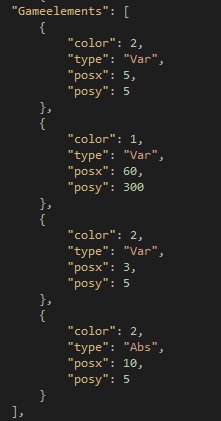
\includegraphics[scale= 0.6]{images/GameelementJson}
		\end{column}
	\end{columns}
	\bigskip
\end{frame}

\begin{frame}
	\frametitle{Aufbau JSON}
	{\center
		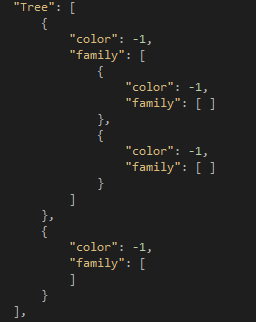
\includegraphics[scale= 0.7]{images/TreeJson}	
		\par
	}
	\bigskip
\end{frame}

\begin{frame}
	\frametitle{Aufbau JSON}
	\begin{columns}[T]
		\begin{column}{5 cm}
			\begin{itemize}
				\item Auswertungsstruktur
				\item Attribute
				\begin{itemize}
					\item color: Dummy-Objekt
					\item family: Verschachtelung
				\end{itemize}
			\end{itemize}
		\end{column}
		\hfill
		\begin{column}{5 cm}
			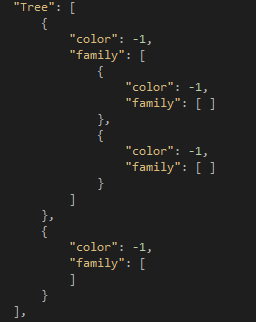
\includegraphics[scale= 0.6]{images/TreeJson}
		\end{column}
	\end{columns}
	\bigskip
\end{frame}

\begin{frame}
	\frametitle{Aufbau Json}
	{\center
		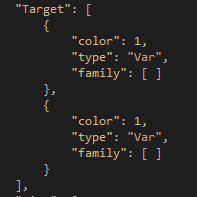
\includegraphics[scale= 1]{images/TargetJson}	
		\par
	}
	\bigskip
\end{frame}

\begin{frame}
	\frametitle{Aufbau JSON}
	\begin{columns}[T]
		\begin{column}{5 cm}
			\begin{itemize}
				\item Zielkonstellation
				\item Baumstruktur
				\item Attribute
				\begin{itemize}
					\item color: Farbgruppe
					\item type: Typ des Objekts
					\item family: Verschachtelung
				\end{itemize}
			\end{itemize}
		\end{column}
		\hfill
		\begin{column}{5 cm}
			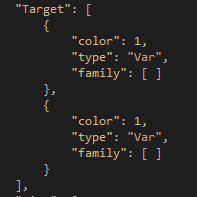
\includegraphics[scale= 0.9]{images/TargetJson}
		\end{column}
	\end{columns}
	\bigskip
\end{frame}

\begin{frame}
	\frametitle{Aufbau JSON}
	{\center
		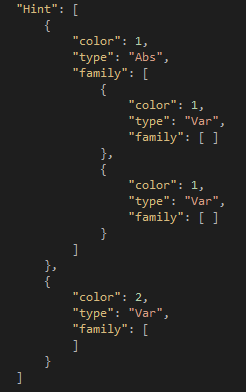
\includegraphics[scale= 0.65]{images/HintJson}	
		\par
	}
	\bigskip
\end{frame}

\begin{frame}
	\frametitle{Aufbau JSON}
	\begin{columns}[T]
		\begin{column}{5cm}
			\begin{itemize}
				\item Hinweis zum Ziel
				\item Baumstruktur
				\item Attribute
				\begin{itemize}
					\item color: Farbgruppe
					\item type: Typ des Objekts
					\item family: Verschachtelung
				\end{itemize}
			\end{itemize}
		\end{column}
		\hfill
		\begin{column}{4.5cm}
			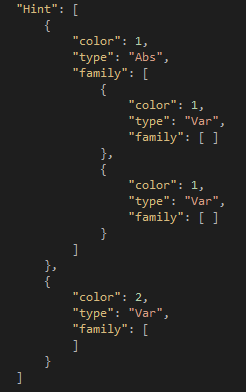
\includegraphics[scale= 0.65]{images/HintJson}
		\end{column}
	\end{columns}
	\bigskip
\end{frame}

\begin{frame}
	\frametitle{Beispiel}
		{\center
			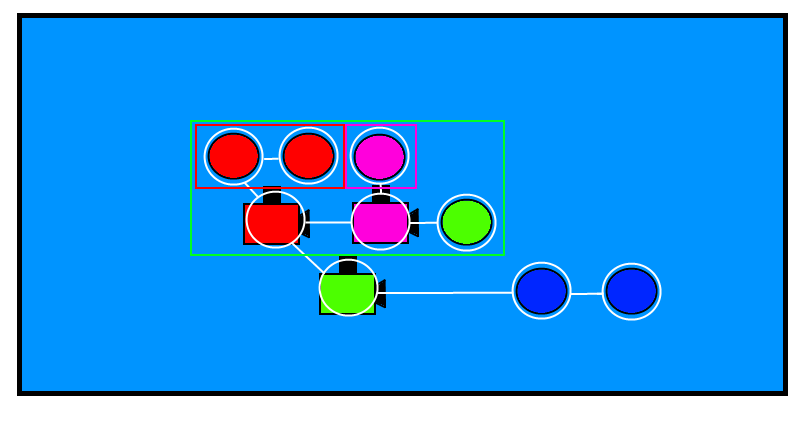
\includegraphics[scale= 0.55]{images/AuswertungVertex}	
			\par
		}
	\bigskip
\end{frame}

\begin{frame}
	\frametitle{Beispiel}
	{\center
		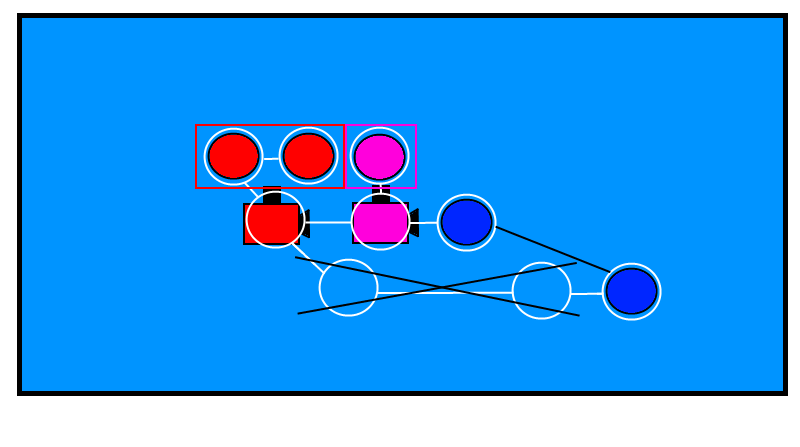
\includegraphics[scale= 0.55]{images/AuswertungVertex2}	
		\par
	}
	\bigskip
\end{frame}

\begin{frame}
	\frametitle{Beispiel}
	{\center
		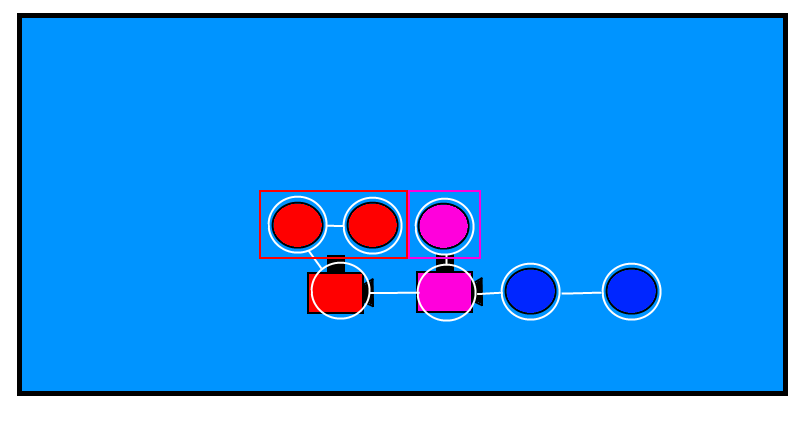
\includegraphics[scale= 0.55]{images/AuswertungVertex3}	
		\par
	}
	\bigskip
\end{frame}

\begin{frame}
	\frametitle{Sequenzdiagramm Auswertung}
	{\center
		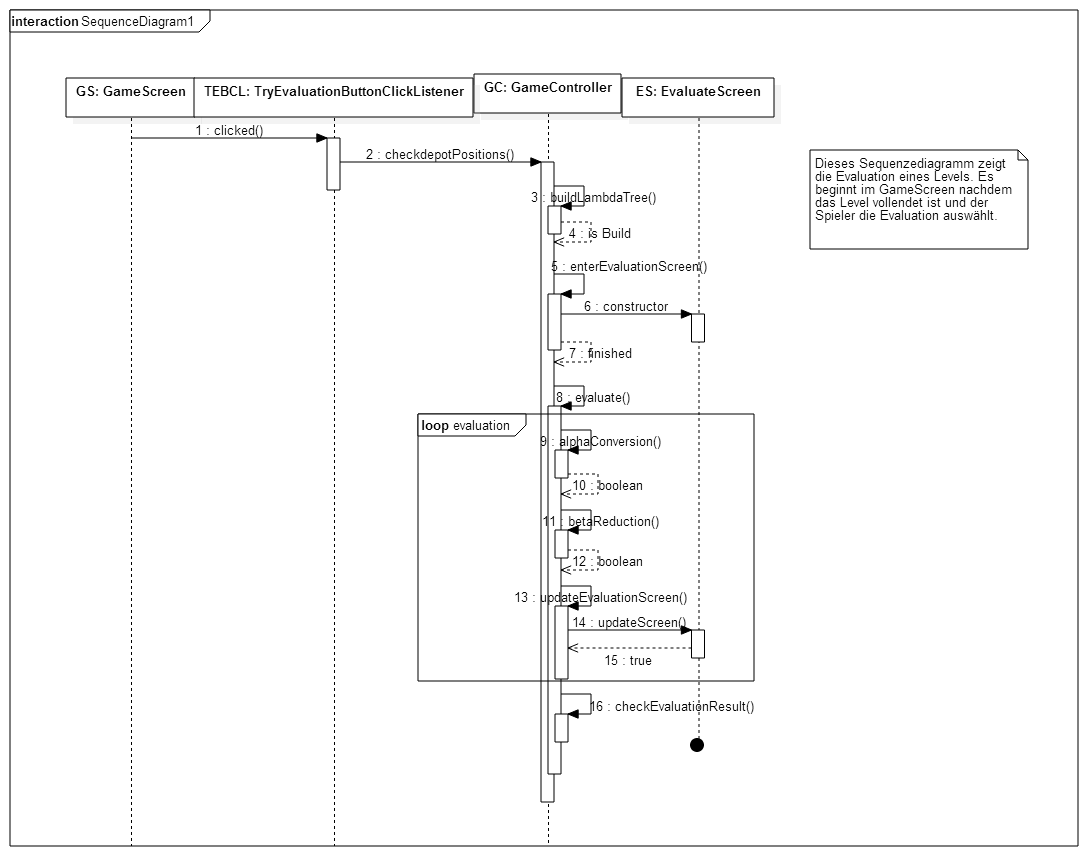
\includegraphics[scale= 0.23]{images/SequenzdiagrammAuswertung}	
		\par
	}
	\bigskip
\end{frame}

\section{Datenbank}
\begin{frame}
	\frametitle{Datenbank Model}
	\begin{itemize}
		\item SQLite Datenbank
		\item Speichert:
		\begin{itemize}
			\item Einstellungen
			\item Profilinformationen
			\item Spielfortschritt
			\item Spiel-Statistiken
		\end{itemize}
	\end{itemize}
	\bigskip
\end{frame}

\section{Ende}
\begin{frame}
	\huge
	Vielen Dank für Ihre Aufmerksamkeit!
\end{frame}

\end{document}
